\documentclass{standalone}
\usepackage[dvipsnames,svgnames,x11names]{xcolor}
\usepackage{tikz}
\usepackage{pgfplots}
\pgfplotsset{compat = 1.12}
\usepackage{../thesismath}
\begin{document}
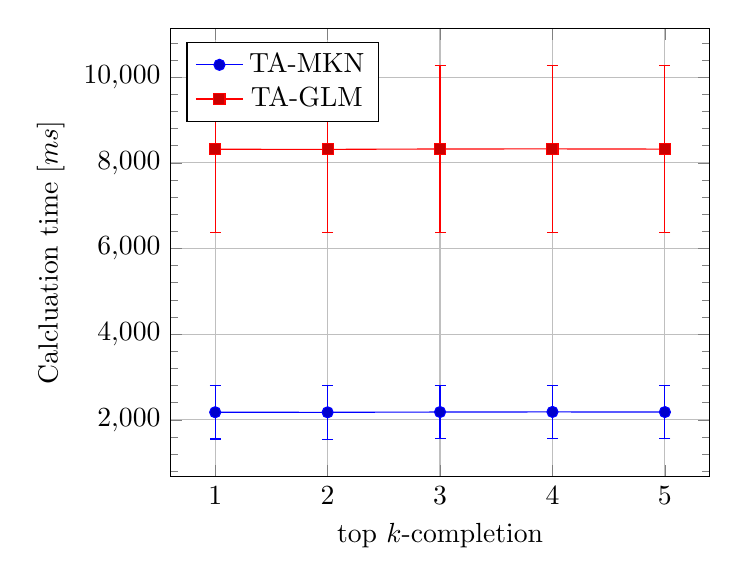
\begin{tikzpicture}[baseline]

\begin{axis}[
  xlabel = {top $k$-completion},
  xtick = {1, ..., 5},
  ylabel = {Calcluation time [$m s$]},
  scaled ticks = false,
  minor y tick num = 4,
  grid = major,
  legend entries = {{TA-MKN}, {TA-GLM}, {NRA-MKN}, {NRA-GLM}, {SMPL-MKN}, {SMPL-GLM}},
  legend pos = north west,
]

% over 100 test sequences on my own machine

% SMPL-MKN
\addplot+[
  error bars/.cd,
  y dir = both,
  y explicit,
] table [y error = us_error] {
  n us       us_error
  1 2178.157  625.296
  2 2176.596  626.603
  3 2183.488  625.449
  4 2185.850  624.627
  5 2182.684  625.372
};

% SMPL-GLM
\addplot+[
  error bars/.cd,
  y dir = both,
  y explicit,
] table [y error = us_error] {
  n us       us_error
  1 8315.938 1941.474
  2 8313.401 1943.088
  3 8322.613 1945.171
  4 8323.701 1945.066
  5 8320.141 1944.259
};

\end{axis}

\end{tikzpicture}
\end{document}
